\section{Продвинутые Policy Gradient}\label{TRPOPPOsection}

\subsection{Суррогатная функция}

Как можно хотя бы частично побороться с ключевой проблемой Policy Gradient подхода --- с on-policy режимом? Есть два соображения, как это можно попробовать сделать.

Во-первых, можно попробовать вместо градиентного подъёма использовать какой-то более тяжеловесный метод оптимизации, например, методы оптимизации второго порядка. Такие методы обычно требуют меньше обращений к оракулу, делая меньше итераций, за счёт более высокой вычислительной сложности каждого шага. В нашем случае это может быть ровно то, что нам нужно --- вызов оракула для нас это сбор данных, и какие-то дополнительные вычисления <<на компьютере>> можно считать дешёвой процедурой. 

Вторая идея --- можно как-то попробовать посчитать оценку градиента в точке текущих параметров, при этом используя сэмплы, полученные при помощи другой стратегии. Полностью перейти в off-policy режим с сохранением всех преимуществ on-policy у нас не получится, поэтому придётся наложить ограничение на эту другую стратегию сбора данных: она должна быть очень похожей версией оцениваемой стратегии, то есть, можно считать, недавней версии актуальной стратегии. То, что стратегия сбора данных <<похожа>> на текущую, означает, что её траектории тоже в некотором смысле <<похожи>>: понятно, что это важно, ведь много информации о градиенте политики по около-оптимальным параметрам с траекторий случайного агента собрать не получится, просто потому что такие траектории у около-оптимальной стратегии почти не встретятся.

На самом деле эти две идеи примерно об одном и том же, что мы и увидим далее.

Итак, допустим мы хотим оптимизировать стратегию $\textcolor{ChadBlue}{\pi_\theta}$ по параметрам $\textcolor{ChadBlue}{\theta}$, используя только сэмплы из другой стратегии $\textcolor{ChadPurple}{\pi^{\old}}$ (в итоговой схеме это будет недавняя версия стратегии). Что нам тогда мешает оценить значение \eqref{advantagepg}?

$$
\nabla_{\theta} J(\pi) = \frac{1}{1 - \gamma}\E_{\textcolor{ChadBlue}{d_\pi}(s)} \E_{\textcolor{ChadBlue}{\pi}(a \mid s)} \nabla_{\theta} \log \textcolor{ChadBlue}{\pi_\theta} (a \mid s) \textcolor{ChadBlue}{A^{\pi}}(s, a)
$$

Во-первых, у нас нет сэмплов из $\textcolor{ChadBlue}{d_\pi}(s)$, ведь в данных есть только\footnote{с учётом забивания на $\gamma^t$ и наших прочих оговорок; но для корректности выкладок будем в этой главе писать везде дисконтированные частоты посещения состояний $d$} состояния из $\textcolor{ChadPurple}{d_{\pi^{\old}}}(s)$. Мы уже обсуждали, что поскольку формула говорит проводить policy improvement, мы можем подменить это распределение на любое другое, и схема останется рабочей. Однако ключевой является вторая проблема. У нас нет оценки $\textcolor{ChadBlue}{A^{\pi}}(s, a)$. Если мы попробуем оценить Advantage для одной стратегии по данным из другой, то нам придётся вводить все те коррекции, которые мы обсуждали в разделе \ref{subsec:retrace} про Retrace оценку, которая скорее всего схлопнется в смещённую. Очень хотелось бы всё-таки оставить <<чистую>> GAE-оценку, то есть как-то использовать <<несвежего>> критика  $\textcolor{ChadPurple}{A^{\pi^{\old}}}(s, a)$ в формуле градиента.

% В принципе, мы можем сделать это напрямую через importance sampling:
% $$
% \nabla_{\theta} J(\textcolor{ChadBlue}{\theta}) = \E_{\Traj \sim \textcolor{ChadPurple}{\pi^{\old}}} \frac{\mathcal{P}(\Traj \mid \textcolor{ChadBlue}{\pi_{\theta}})}{\mathcal{P}(\Traj \mid \textcolor{ChadPurple}{\pi^{\old}})} \sum_{t \ge 0} \nabla_{\theta} \log \textcolor{ChadBlue}{\pi_{\theta}}(a_t \mid s_t) \textcolor{ChadBlue}{A^\pi}(s_t, a_t)
% $$
% Появившийся коэффициент в принципе вычислим, поскольку вероятности переходов (которые мы не знаем) сокращаются:
% $$\frac{\mathcal{P}(\Traj \mid \textcolor{ChadBlue}{\pi_\theta})}{\mathcal{P}(\Traj \mid \textcolor{ChadPurple}{\pi^{\old}})} = \frac{\prod\limits_{t \ge 0} \textcolor{ChadBlue}{\pi_\theta}(a_t \mid s_t)}{\prod\limits_{t \ge 0} \textcolor{ChadPurple}{\pi^{\old}}(a_t \mid s_t)}$$
% Но, конечно, этот коэффициент ужасен: он может быть экспоненциально большим или маленьким и скорее всего затухнет или взорвётся. Поколдовать тут особо не получится, поскольку скорее всего мини-батч любого разумного размера будет доминироваться одной парой $s_t, a_t$ с самым большим значением коэффициента, и никакой стабильной процедурой оптимизации тут не пахнет. Нужно подойти с другой стороны...

Как сделать так, чтобы у нас где-то в формулах образовался <<несвежий>> критик? На помощь приходит RPI, формула \eqref{RPI}: мы можем сменить функцию награды на Advantage функцию любой другой стратегии! Давайте запишем это в следующем виде:

\begin{proposition}
\,
\begin{equation}\label{RPIdecoupled}
J(\textcolor{ChadBlue}{\pi_{\theta}}) = J(\textcolor{ChadPurple}{\pi^{\old}}) + \frac{1}{1 - \gamma}\E_{s \sim \textcolor{ChadBlue}{d_{\pi_{\theta}}}(s)} \E_{a \sim \textcolor{ChadBlue}{\pi_{\theta}}(a \mid s)} \textcolor{ChadPurple}{A^{\pi^{\old}}}(s_t, a_t)
\end{equation}
\begin{proof}
Из RPI \eqref{RPI} следует, что для любых двух стратегий верно 
$$J(\textcolor{ChadBlue}{\pi_{\theta}}) = J(\textcolor{ChadPurple}{\pi^{\old}}) + \E_{\Traj \sim \textcolor{ChadBlue}{\pi_{\theta}}} \sum_{t \ge 0} \gamma^t \textcolor{ChadPurple}{A^{\pi^{\old}}}(s_t, a_t)$$
Для получения формулы достаточно переписать мат.ожидание по траекториям из $\textcolor{ChadBlue}{\pi_{\theta}}$ через state visitation distribution, подставив в теореме \ref{th:decoupling_stoch} в качестве $f(s, a) \HM= \textcolor{ChadPurple}{A^{\pi^{\old}}}(s, a)$.
\end{proof}
\end{proposition}

Тогда градиент исходного функционала $\textcolor{ChadBlue}{\nabla_\theta} J(\textcolor{ChadBlue}{\pi_{\theta}})$ есть градиент правой части, и в ней уже как-то <<замешана>> оценка Advantage для стратегии $\textcolor{ChadPurple}{\pi^{\old}}$, которое мы сможем посчитать при помощи GAE-оценки:

$$\textcolor{ChadBlue}{\nabla_\theta} J(\textcolor{ChadBlue}{\pi_{\theta}}) = \textcolor{ChadBlue}{\nabla_\theta} \frac{1}{1 - \gamma}\E_{s \sim \textcolor{ChadBlue}{d_{\pi_{\theta}}}(s)} \E_{a \sim \textcolor{ChadBlue}{\pi_{\theta}}(a \mid s)} \textcolor{ChadPurple}{A^{\pi^{\old}}}(s_t, a_t)$$

Мы также можем справиться с мат.ожиданием $\E_{a \sim \textcolor{ChadBlue}{\pi_{\theta}}(a \mid s)}$ при помощи importance sampling. Да, этот коэффициент может быть ужасен (сильно большим единицы или близким к нулю), но это коррекция всего лишь за один шаг, и такая дробь будет терпимой.

\begin{equation}\label{perfectsurrogate}
\textcolor{ChadBlue}{\nabla_\theta} J(\textcolor{ChadBlue}{\pi_{\theta}}) = \textcolor{ChadBlue}{\nabla_\theta} \frac{1}{1 - \gamma} \E_{s \sim \textcolor{ChadBlue}{d_{\pi_{\theta}}}(s)} \E_{a \sim \textcolor{ChadPurple}{\pi^{\old}}(a \mid s)} \frac{\textcolor{ChadBlue}{\pi_{\theta}}(a \mid s)}{\textcolor{ChadPurple}{\pi^{\old}}(a \mid s)} \textcolor{ChadPurple}{A^{\pi^{\old}}}(s_t, a_t)
\end{equation}

Осталась последняя проблема: $\textcolor{ChadBlue}{d_{\pi_{\theta}}}(s)$. В роллаутах, сгенерированных при помощи $\textcolor{ChadPurple}{\pi^{\old}}$, состояния всё-таки будут приходить из $\textcolor{ChadPurple}{d_{\pi^{\old}}}(s)$, и тут мы importance sampling не сделаем даже при большом желании, так как просто не можем внятно оценить эти величины: из частот посещения состояний мы можем только сэмплировать.

Рассмотрим аппроксимацию: что, если мы в формуле \eqref{perfectsurrogate} заменим $\textcolor{ChadBlue}{d_{\pi_{\theta}}}(s)$ на $\textcolor{ChadPurple}{d_{\pi^{\old}}}(s)$? Это, вообще говоря, будет какая-то другая функция.

\begin{definition}
Введём суррогатную функцию:
\begin{equation}\label{surrogate}
L_{\textcolor{ChadPurple}{\pi^{\old}}}(\textcolor{ChadBlue}{\theta}) \coloneqq \frac{1}{1 - \gamma}\E_{s \sim \textcolor{ChadPurple}{d_{\pi^{\old}}}(s)} \E_{a \sim \textcolor{ChadPurple}{\pi^{\old}}(a \mid s)} \frac{\textcolor{ChadBlue}{\pi_\theta}(a \mid s)}{\textcolor{ChadPurple}{\pi^{\old}}(a \mid s)} \textcolor{ChadPurple}{A^{\pi^{\old}}}(s, a)   
\end{equation}
\end{definition}

\begin{proposition}
Сэмплы из мат.ожиданий в суррогатной функции --- это сэмплы из роллаутов, сгенерированных при помощи $\textcolor{ChadPurple}{\pi^{\old}}$:
\begin{equation*}
L_{\textcolor{ChadPurple}{\pi^{\old}}}(\textcolor{ChadBlue}{\theta}) = \E_{\Traj \sim \textcolor{ChadPurple}{\pi^{\old}}} \sum_{t \ge 0} \gamma^t \frac{\textcolor{ChadBlue}{\pi_\theta}(a \mid s)}{\textcolor{ChadPurple}{\pi^{\old}}(a \mid s)} \textcolor{ChadPurple}{A^{\pi^{\old}}}(s, a)
\end{equation*}
\begin{proof}[Пояснение]
Применить теорему \ref{th:decoupling_stoch} в обратную сторону для $f(s, a) \HM= \frac{\textcolor{ChadBlue}{\pi_\theta}(a \mid s)}{\textcolor{ChadPurple}{\pi^{\old}}(a \mid s)} \textcolor{ChadPurple}{A^{\pi^{\old}}}(s, a)$
\end{proof}
\end{proposition}

Какой у этой суррогатной функции $L_{\textcolor{ChadPurple}{\pi^{\old}}}(\textcolor{ChadBlue}{\theta})$ физический смысл? Мы сказали, что наши настраиваемые параметры $\textcolor{ChadBlue}{\theta}$ не влияют на частоты посещения состояний, то есть выбор действий не влияет на то, какие состояния мы будем посещать в будущем. Это очень сильное допущение, поэтому аппроксимация не самая удачная. Давайте поймём, что будет происходить, если мы будем оптимизировать вместо честного, исходного функционала, такую суррогатную функцию при фиксированной $\textcolor{ChadPurple}{\pi^{\old}}$:
\begin{equation}\label{surrogate_opt}
L_{\textcolor{ChadPurple}{\pi^{\old}}}(\textcolor{ChadBlue}{\theta}) \to \max_{\textcolor{ChadBlue}{\theta}}
\end{equation}

\begin{proposition}\label{prop:surrogateoptispi}
Решением оптимизационной задачи \eqref{surrogate_opt} является жадная стратегия по отношению к $\textcolor{ChadPurple}{Q^{\pi^{\old}}}(s, a)$ (или, что тоже самое, к Advantage-функции стратегии $\textcolor{ChadPurple}{\pi^{\old}}$):
$$\textcolor{ChadBlue}{\pi_\theta}(s) = \argmax_{a} \textcolor{ChadPurple}{A^{\pi^{\old}}}(s, a)$$

\begin{proof}
Эта оптимизационная задача распадается на оптимизационную задачу для каждого $s$, а решением задачи
$$\E_{a \sim \textcolor{ChadPurple}{\pi^{\old}}(a \mid s)} \frac{\textcolor{ChadBlue}{\pi_\theta}(a \mid s)}{\textcolor{ChadPurple}{\pi^{\old}}(a \mid s)} \textcolor{ChadPurple}{A^{\pi^{\old}}}(s, a) = \E_{a \sim \textcolor{ChadBlue}{\pi_\theta}(a \mid s)} \textcolor{ChadPurple}{A^{\pi^{\old}}}(s, a) \to \max_{\textcolor{ChadBlue}{\theta}}$$
является <<жадная>> стратегия.
\end{proof}
\end{proposition}

Другими словами, такая суррогатная функция просто говорит проводить policy improvement стратегии $\textcolor{ChadPurple}{\pi^{\old}}$, но в состояниях, приходящих из частот посещения состояний $\textcolor{ChadPurple}{d_{\pi^{\old}}}(s)$. Такая очередная форма нам сейчас будет удобна, поскольку такая суррогатная функция является локальной аппроксимацией нашего оптимизируемого функционала, причём эта аппроксимация --- не просто, скажем, линейное приближение оптимизируемой функции, а какое-то более умное, учитывающее особенности задачи. 

\subsection{Нижняя оценка}

Итак, у нас есть аппроксимация нашего оптимизируемого функционала через суррогатную функцию, с которой мы можем работать:
$$J(\textcolor{ChadBlue}{\pi}) \approx J(\textcolor{ChadPurple}{\pi^{\old}}) + L_{\textcolor{ChadPurple}{\pi^{\old}}}(\textcolor{ChadBlue}{\theta}) = J(\textcolor{ChadPurple}{\pi^{\old}}) + \frac{1}{1 - \gamma}\E_{s \sim \textcolor{ChadPurple}{d_{\pi^{\old}}}(s)} \E_{a \sim \textcolor{ChadPurple}{\pi^{\old}}(a \mid s)} \frac{\textcolor{ChadBlue}{\pi_\theta}(a \mid s)}{\textcolor{ChadPurple}{\pi^{\old}}(a \mid s)} \textcolor{ChadPurple}{A^{\pi^{\old}}}(s, a)$$

Насколько эта аппроксимация хороша? Наша интуиция была в том, что если $\textcolor{ChadBlue}{\pi}$ <<похожа>> на $\textcolor{ChadPurple}{\pi^{\old}}$, то частоты посещения состояний у них тоже наверняка будут похожи. Формализовать <<похожесть>> стратегий можно, например, так:
\begin{definition}
Введём расстояние между стратегиями $\textcolor{ChadPurple}{\pi^{\old}}, \textcolor{ChadBlue}{\pi_\theta}$ как среднюю KL-дивергенцию между ними по состояниям из частот посещения первой стратегии:
$$\KL(\textcolor{ChadPurple}{\pi^{\old}} \parallel \textcolor{ChadBlue}{\pi_\theta}) \coloneqq \E_{s \sim \textcolor{ChadPurple}{d_{\pi^{\old}}}(s)} \KL(\textcolor{ChadPurple}{\pi^{\old}}(a \mid s) \parallel \textcolor{ChadBlue}{\pi_\theta}(a \mid s))$$
\end{definition}

\begin{theoremBox}[label=th:Lapproximationestimation]{}
\,
\begin{equation*} 
\left| J(\textcolor{ChadBlue}{\pi_\theta}) - J(\textcolor{ChadPurple}{\pi^{\old}}) - L_{\textcolor{ChadPurple}{\pi^{\old}}}(\textcolor{ChadBlue}{\theta}) \right| \le C \sqrt{\KL(\textcolor{ChadPurple}{\pi^{\old}} \parallel \textcolor{ChadBlue}{\pi_\theta}) }
\end{equation*}
где $C$ --- константа, равная $C \HM= \frac{\sqrt{2} \gamma}{(1 - \gamma)^2} \max\limits_{s, a} |\textcolor{ChadPurple}{A^{\pi^{\old}}}(s, a)|$
\begin{proof}[Без доказательства; интересующиеся могут обратиться к статье \href{https://arxiv.org/pdf/1705.10528.pdf}{Constrained Policy Optimization}]
\end{proof}
\end{theoremBox}

Конечно, это очень грубая оценка, хотя бы потому, что она верна для произвольных MDP и произвольных двух стратегий. Но ключевой момент в том, что мы теперь формально можем вывести \emph{нижнюю оценку} (lower bound) на оптимизируемый функционал\footnote{исторически в статьях по TRPO и PPO использовалась чуть более грубая нижняя оценка, в которой ошибка между суррогатной функцией и честным функционалом оценивалась сверху при помощи KL-дивергенции в максимальной форме:
$$\KL^{\max}(\textcolor{ChadPurple}{\pi^{\old}} \parallel \textcolor{ChadBlue}{\pi}) \coloneqq \max_s \KL(\textcolor{ChadPurple}{\pi^{\old}}(a \mid s) \parallel \textcolor{ChadBlue}{\pi_\theta}(a \mid s))$$
Однако такое выражение посчитать в практических алгоритмах нельзя, поэтому далее её приходилось эвристически заменять на среднее по $s \HM\sim \textcolor{ChadPurple}{d_{\pi^{\old}}}(s)$. Уточнённая нижняя оценка обосновывает этот переход и указывает, что из KL-дивергенции также нужно взять корень; в остальном на ход дальнейших рассуждений это не влияет.
}:
\begin{theorem}[Performance Lower Bound]
\begin{equation}\label{lowerbound}
J(\textcolor{ChadBlue}{\pi_\theta}) - J(\textcolor{ChadPurple}{\pi^{\old}}) \ge L_{\textcolor{ChadPurple}{\pi^{\old}}}(\textcolor{ChadBlue}{\theta}) - C \sqrt{\KL(\textcolor{ChadPurple}{\pi^{\old}} \parallel \textcolor{ChadBlue}{\pi_{\theta}})}
\end{equation}
\end{theorem}

Возникает любопытнейшая идея: возможно, мы можем работать не с исходным функционалом, а с нижней оценкой.

\begin{theorem}
Процедура оптимизации
\begin{equation}\label{lowerboundopt}
\textcolor{ChadBlue}{\theta_{k+1}} \coloneqq \argmax_{\textcolor{ChadBlue}{\theta}} \left[ L_{\textcolor{ChadPurple}{\pi_{\theta_k}}}(\textcolor{ChadBlue}{\theta}) - C \sqrt{\KL(\textcolor{ChadPurple}{\pi_{\theta_k}} \parallel \textcolor{ChadBlue}{\pi_\theta})} \right]
\end{equation}
гарантирует монотонное неубывание функционала: $J(\textcolor{ChadBlue}{\pi_{\theta_{k+1}}}) \ge J(\textcolor{ChadPurple}{\pi_{\theta_{k}}})$
\begin{proof}
В точке $\theta \HM= \theta_k$ суррогатная функция $L_{\pi_{\theta_k}}(\theta)$ равна нулю, поскольку
\begin{align*}
L_{\pi_{\theta_k}}(\theta_k) &= \\
= \{\text{по определению \eqref{surrogate}}\} &= \frac{1}{1 - \gamma}\E_{s \sim d_{\pi_{\theta_{k}}}(s)} \E_{a \sim \pi_{\theta_{k}}(a \mid s)} \frac{\pi_{\theta_{k}}(a \mid s)}{\pi_{\theta_{k}}(a \mid s)} A^{\pi_{\theta_{k}}}(s, a) = \\ 
&= \frac{1}{1 - \gamma}\E_{s \sim d_{\pi_{\theta_{k}}}(s)} \E_{a \sim \pi_{\theta_{k}}(a \mid s)} A^{\pi_{\theta_{k}}}(s, a) = \\
\{\text{следствие RPI \eqref{RPIdecoupled}}\} &= J(\pi_{\theta_{k}}) - J(\pi_{\theta_{k}}) = 0
\end{align*}

Понятно, что $\KL(\pi_{\theta_k} \parallel \pi_\theta)$ в точке $\theta \HM= \theta_k$ тоже равна 0, так как во всех состояниях $\KL$ между одинаковыми стратегиями равна нулю. Значит, максимум нижней оценки не меньше нуля, а она есть нижняя оценка на $J(\textcolor{ChadBlue}{\pi_{\theta_{k+1}}}) -\HM J(\textcolor{ChadPurple}{\pi_{\theta_{k}}})$.
\end{proof}
\end{theorem}

\needspace{9\baselineskip}
\begin{wrapfigure}[9]{r}{0.5\textwidth}
%\vspace{-0.5cm}
\centering
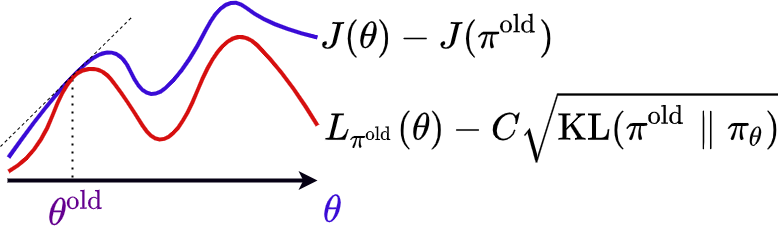
\includegraphics[width=0.5\textwidth]{Images/MM.png}
%\vspace{-0.9cm}
\end{wrapfigure}

Итак, в воздухе витает идея заняться типичным \emph{minorization-maximization} алгоритмом. Сначала мы подтягиваем нашу нижнюю оценку так, чтобы в текущей точке $\theta \HM= \theta^{\old}$ она в точности совпадала с оптимизируемой функцией (minorization). Затем мы начинаем при фиксированном $\textcolor{ChadPurple}{\theta^{\old}}$ оптимизировать по $\textcolor{ChadBlue}{\theta}$ не наш функционал (который мы не сможем оптимизировать без новых сэмплов из новой стратегии $\textcolor{ChadBlue}{\pi_\theta}$ с текущими значениями параметров), а нижнюю оценку, с которой умеем работать (maximization). 

То есть, что мы получили: мы <<можем>> оптимизировать не $J(\textcolor{ChadBlue}{\pi_\theta}) \HM- J(\textcolor{ChadPurple}{\pi^{\old}})$ по формуле \eqref{perfectsurrogate}, а нашу суррогатную функцию $L_{\textcolor{ChadPurple}{\pi^{\old}}}(\textcolor{ChadBlue}{\theta})$, то есть проводить policy improvement стратегии $\textcolor{ChadPurple}{\pi^{\old}}$, но добавив штраф --- регуляризатор --- за различие между $\textcolor{ChadBlue}{\pi_\theta}$ и стратегией, из которой приходят данные $\textcolor{ChadPurple}{\pi^{\old}}$:

\begin{equation}\label{lowerboundmean}
L_{\textcolor{ChadPurple}{\pi^{\old}}}(\textcolor{ChadBlue}{\theta}) - C \sqrt{\KL(\textcolor{ChadPurple}{\pi^{\old}} \parallel \textcolor{ChadBlue}{\pi_\theta}) } \to \max_{\textcolor{ChadBlue}{\theta}}
\end{equation}

Мы получили процедуру, гарантирующую улучшение стратегии, что звучит подозрительно хорошо. Очень похожие гарантии улучшения стратегии у нас были в policy improvement. Интересно порассуждать, в чём отличие. Мы уже увидели в утверждении \ref{prop:surrogateoptispi}, что оптимизация суррогатной функции без регуляризатора соответствует policy improvement-у стратегии $\textcolor{ChadPurple}{\pi^{\old}}$. Однако как мы помним, жадный policy improvement вовсе не является наилучшим: если мы в некотором состоянии $s$ перекладываем вероятностную массу в какое-то действие, чтобы увеличить среднее значение $\textcolor{ChadPurple}{A^{\pi^{\old}}}(s, a)$, мы попадаем чаще в те состояния, где стратегия $\textcolor{ChadPurple}{\pi^{\old}}$ набирает больше, да, но на самом деле мы таким изменением стратегии можем помешать себе добираться чаще до тех состояний, где $\textcolor{ChadPurple}{A^{\pi^{\old}}}(s, a)$ принимает большие положительные значения!

\begin{exampleBox}[righthand ratio=0.4, sidebyside, sidebyside align=center, lower separated=false]{}
Что говорит policy improvement для MDP с картинки и заданной стратегией $\textcolor{ChadPurple}{\pi^{\old}}$? В начальном состоянии $\textcolor{ChadPurple}{Q^{\pi^{\old}}}(s, \colorsquare{ChadBlue}) \HM= +10$, $\textcolor{ChadPurple}{Q^{\pi^{\old}}}(s, \colorsquare{ChadRed}) \HM= -100$, и поэтому улучшение будет заключаться в том, что новая стратегия должна чаще выбирать именно действие $\colorsquare{ChadBlue}$, выбирать +10. Это связано с тем, что policy improvement игнорирует влияние действий на частоты посещения состояний, и оптимизирует <<новую награду>> $\textcolor{ChadPurple}{A^{\pi^{\old}}}(s, a)$ независимо в каждом состоянии жадным образом. Он не видит, что выбор в начальном состоянии действия $\colorsquare{ChadRed}$ позволит ему попасть в такое состояние, где для одного из действий $\textcolor{ChadPurple}{A^{\pi^{\old}}}(s_2, \colorsquare{ChadBlue}) \HM= +200$!

\tcblower
\vspace{-0.2cm}
\begin{adjustwidth}{-0.35cm}{0cm}
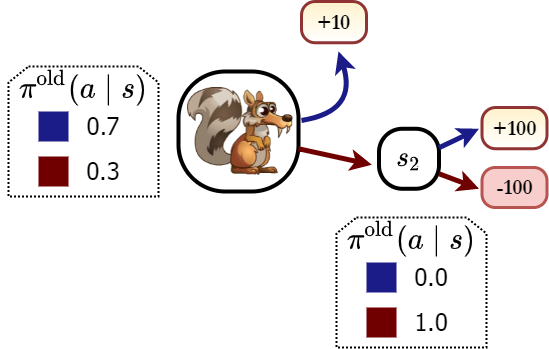
\includegraphics[width=\textwidth]{Images/GreedyPIisBad.png}
\end{adjustwidth}
\end{exampleBox}

Поэтому формула policy gradient --- <<наилучшего policy improvement-а>> --- говорит, что как только параметры $\textcolor{ChadBlue}{\theta}$ хоть чуть-чуть изменяются, сразу же стоит улучшать новую стратегию, то есть использовать свежего критика. Мы же свежего критика получить не можем, хотим пользоваться лишь <<несвежим>> $\textcolor{ChadPurple}{A^{\pi^{\old}}}(s, a)$, и нижняя оценка \eqref{lowerboundmean} даёт промежуточную альтернативу, что тогда можно делать: добавить регуляризатор, запрещающий сильное изменение исходной стратегии $\textcolor{ChadPurple}{\pi^{\old}}$.

Однако чтобы оптимизировать \eqref{lowerboundmean}, нужно как-то определить значение константы $C$: мы не умеем считать выражение для неё из теоремы \ref{th:Lapproximationestimation}, поскольку там присутствует максимум Advantage-функции по всем парам состояние-действие\footnote{мы могли бы оценить его сверху как $2R^{\max}$, где $R^{\max}$ --- максимальная награда, но это было бы непрактично грубой оценкой.}. Мы можем заменить его на гиперпараметр, но, чтобы не потерять теоретические гарантии, он должен быть достаточно большим, чтобы превосходить значение из теоремы. Вообще, скорее всего, даже если бы мы знали эту константу, она была бы колоссальной: чего стоит только $(1 \HM- \gamma)^2$ в знаменателе формулы из теоремы \ref{th:Lapproximationestimation}. Поэтому практической пользы от такой нижней оценки всё равно много бы не было: её оптимизация делала бы слишком консервативные шаги обновления политики.

% Проблемы на этом не заканчиваются: мы не умеем считать меру схожести стратегий $\KL^{\max}$, поскольку невозможно взять максимум по состояниям. Предлагается тихонько заменить максимум на среднее по состояниям\footnote{позже в статье \href{https://arxiv.org/abs/1705.10528}{Constrained Policy Optimization} удалось доказать похожую на теорему \ref{th:Lapproximationestimation} оценку, в которой использовалось именно среднее KL-дивергенции по состояниям; разве что, KL-дивергенция в этой оценке находится под квадратным корнем. Поэтому эту замену можно считать обоснованной.}:
% $$\max_s \KL(\textcolor{ChadPurple}{\pi^{\old}}(a \mid s) \parallel \textcolor{ChadBlue}{\pi_\theta}(a \mid s)) \approx \E_{s \sim \textcolor{ChadPurple}{d_{\pi^{\old}}}(s)} \KL(\textcolor{ChadPurple}{\pi^{\old}}(a \mid s) \parallel \textcolor{ChadBlue}{\pi_\theta}(a \mid s))$$

% Среднее берём по состояним из $\textcolor{ChadPurple}{d_{\pi^{\old}}}(s)$ исключительно из удобства, так как именно из него будут приходить состояния в роллаутах, сгенерированных $\textcolor{ChadPurple}{\pi^{\old}}$. Везде далее будем для сокращения использовать такую запись:
% $$\KL(\textcolor{ChadPurple}{\pi^{\old}} \parallel \textcolor{ChadBlue}{\pi_\theta}) \coloneqq \E_{s \sim \textcolor{ChadPurple}{d_{\pi^{\old}}}(s)} \KL(\textcolor{ChadPurple}{\pi^{\old}}(a \mid s) \parallel \textcolor{ChadBlue}{\pi_\theta}(a \mid s))$$ 



\subsection{Trust Region Policy Optimization (TRPO)}

В TRPO предлагается воспользоваться полученной теорией, чтобы построить на основе идеи суррогатной функции более <<мощный>> метод оптимизации, чем обычный градиентный спуск. Как обычно устроены методы оптимизации? В текущей точке для рассматриваемой функции строится какая-то модель, какая-то локально верная аппроксимация (например, линейная или квадратичная). Далее эта модель либо оптимизируется, и алгоритм сдвигает текущее решение в сторону оптимума модели (такие методы относят к \emph{line search} подходу), либо модель оптимизируется в некотором <<\emph{регионе доверия}>> (trust region), где эта модель, считается, более-менее похожа на исходный функционал. Подход на основе регионов доверия считается более тяжеловесным, поскольку требует решать на каждом шаге работы алгоритма условную задачу оптимизации, зато более эффективным по числу итераций.

\begin{wrapfigure}{r}{0.2\textwidth}
\vspace{-0.5cm}
\centering
\includegraphics[width=0.2\textwidth]{Images/HardTrustRegion.png}
\vspace{-0.9cm}
\end{wrapfigure}

Основная идея TRPO заключается в переходе от оптимизации \eqref{lowerboundmean} без ограничений к задаче оптимизации с ограничением в trust region форме:
\begin{equation}\label{trustregion}
\begin{cases}
L_{\textcolor{ChadPurple}{\pi^{\old}}}(\textcolor{ChadBlue}{\theta}) \to \max\limits_{\textcolor{ChadBlue}{\theta}} \\
\KL(\textcolor{ChadPurple}{\pi^{\old}} \parallel \textcolor{ChadBlue}{\pi_\theta}) \le \delta
\end{cases}
\end{equation}

То есть, суррогатная функция является локальной аппроксимацией нашего функционала, поэтому на каждом шаге работы алгоритма мы будем работать с ней. При этом второе слагаемое оптимизируемой нижней оценки \eqref{lowerboundmean} подсказывает, что с ростом KL-дивергенции <<нечестный>> функционал всё меньше похож на настоящий, и к нему <<всё меньше доверия>>. Условная задача оптимизации говорит, что оптимизировать суррогатную функцию вместо настоящего функционала можно, но с жёстким ограничением на длину шага.

Вообще говоря, мы получили задачу для оптимизации $L_{\textcolor{ChadPurple}{\pi^{\old}}}(\textcolor{ChadBlue}{\theta})$ методом \emph{натуральных градиентов} (natural gradient): мы оптимизируем функцию, разрешая не шаг некоторой длины по градиенту в пространстве параметров, а шаг некоторой длины в пространстве параметрически заданных распределений. Подробнее о натуральном градиенте можно прочитать в приложении \ref{appendix:ng}. Если раньше градиентный шаг мог сильно поменять стратегию (как распределение в пространстве действий), при том что для других небольших изменений распределения было бы необходимо сильно менять параметры $\textcolor{ChadBlue}{\theta}$, то здесь $\delta$ ограничивает изменение самой стратегии в терминах $\KL$-дивергенции. Ограничение $\delta$ нам при этом всё равно нужно будет выбрать, это аналог learning rate в <<trust region формах>> методов оптимизации.

Как будем задачу \eqref{trustregion} решать? В контексте нашей задачи мы собрали при помощи текущей стратегии некоторое количество данных для Монте-Карло оценок всех мат.ожиданий (в этот момент $\pi^{\old} \HM= \pi_\theta$) и хотим решить задачу \eqref{trustregion}, зафиксировав $\textcolor{ChadPurple}{\pi^{\old}}$ и оптимизируя параметры $\textcolor{ChadBlue}{\theta}$. Обозначим параметры $\textcolor{ChadPurple}{\pi^{\old}}$ как $\textcolor{ChadPurple}{\theta^{\old}}$. Аппроксимируем оптимизируемый функционал $L_{\textcolor{ChadPurple}{\pi^{\old}}}(\textcolor{ChadBlue}{\theta})$ разложением Тейлора до первого порядка с центром в точке $\theta = \theta^{\old}$, а ограничение --- до второго. До второго --- потому что слагаемое первого порядка ноль.

\begin{proposition}
В точке $\theta = \theta^{\old}$ первый член разложения ограничения в ряд Тейлора равен нулю:
\begin{equation*}
\forall s \colon \left. \textcolor{ChadBlue}{\nabla_\theta} \KL(\textcolor{ChadPurple}{\pi^{\old}} \parallel \textcolor{ChadBlue}{\pi_\theta}) \right|_{\theta = \theta^{\old}} = 0
\end{equation*}
\begin{proof}
$\KL$-дивергенция в этой точке равна 0 как среднее по состояниям дивергенций между одинаковыми распределениями, следовательно как функция от $\textcolor{ChadBlue}{\theta}$ она достигает в этой точке глобального минимума $\Rightarrow$ градиент равен нулю.
\end{proof}
% \begin{proof}[Доказательство непосредственной проверкой]
% $$\left. \textcolor{ChadBlue}{\nabla_\theta} \KL(\textcolor{ChadPurple}{\pi^{\old}} \parallel \pi_\theta) \right|_{\theta = \theta^{\old}} = \left. \E_{\textcolor{ChadPurple}{\pi^{\old}}(a \mid s)} \textcolor{ChadBlue}{\nabla_\theta} \log \pi_\theta(a \mid s) \right|_{\theta = \theta^{\old}} = \E_{\pi_{\theta^{\old}}} \textcolor{ChadBlue}{\nabla_\theta} \log \pi_{\theta^{\old}}(a \mid s) = 0$$
% \end{proof}
\end{proposition}

Итак, введём обозначения для предложенного разложения. Пусть $g$ --- градиент $L_{\textcolor{ChadPurple}{\pi^{\old}}}(\textcolor{ChadBlue}{\theta})$ по параметрам $\textcolor{ChadBlue}{\theta}$ в точке $\theta = \theta^{\old}$, а $F$ --- гессиан ограничения в точке $\theta = \theta^{\old}$:
\begin{equation}\label{trpo_gradient}
    g := \left. \textcolor{ChadBlue}{\nabla_\theta} L_{\textcolor{ChadPurple}{\pi^{\old}}}(\textcolor{ChadBlue}{\theta}) \right|_{\theta = \theta^{\old}}
\end{equation}
\begin{equation}\label{trpo_hessian}
    F := \left. \textcolor{ChadBlue}{\nabla^2_\theta} \KL(\textcolor{ChadPurple}{\pi^{\old}} \parallel \textcolor{ChadBlue}{\pi_\theta}) \right|_{\theta = \theta^{\old}}
\end{equation}

В этих обозначениях аппроксимация задачи получается следующая:
\begin{equation}\label{approximatetrustregion}
\begin{cases}
\langle g , \textcolor{ChadBlue}{\theta} - \textcolor{ChadPurple}{\theta^{\old}} \rangle \to \max\limits_{\textcolor{ChadBlue}{\theta}} \\
\frac{1}{2} (\textcolor{ChadBlue}{\theta} - \textcolor{ChadPurple}{\theta^{\old}})^T F (\textcolor{ChadBlue}{\theta} - \textcolor{ChadPurple}{\theta^{\old}}) \le \delta
\end{cases}
\end{equation}

Градиент $g$, на самом деле, весьма любопытен:
\begin{proposition}
Градиент $g$ совпадает с градиентом из алгоритма Advantage Actor Critic \eqref{advantagepg}.
\begin{proof}
\begin{align*}g = \left. \textcolor{ChadBlue}{\nabla_\theta} L_{\textcolor{ChadPurple}{\pi^{\old}}}(\textcolor{ChadBlue}{\theta}) \right|_{\theta = \theta^{\old}} &= \frac{1}{1 - \gamma}\E_{s \sim \textcolor{ChadPurple}{d_{\pi^{\old}}}(s)} \E_{a \sim \textcolor{ChadPurple}{\pi^{\old}}(a \mid s)} \frac{\left. \textcolor{ChadBlue}{\nabla_\theta} \textcolor{ChadBlue}{\pi_\theta}(a \mid s) \right|_{\theta = \theta^{\old}}}{\textcolor{ChadPurple}{\pi^{\old}}(a \mid s)} \textcolor{ChadPurple}{A^{\pi^{\old}}}(s, a) = \\
= \{ \substack{\text{замечаем определение} \\ \text{производной логарифма} }\} &= \frac{1}{1 - \gamma}\E_{s \sim \textcolor{ChadPurple}{d_{\pi^{\old}}}(s)} \E_{a \sim \textcolor{ChadPurple}{\pi^{\old}}(a \mid s)} \left. \textcolor{ChadBlue}{\nabla_\theta} \log \textcolor{ChadBlue}{\pi_\theta}(a \mid s) \right|_{\theta = \theta^{\old}} \textcolor{ChadPurple}{A^{\pi^{\old}}}(s, a)
\end{align*}
что в точности есть градиент обычного ActorCritic c бэйзлайном в точке $\theta = \theta^{\old}$.
\end{proof}
\end{proposition}

\begin{theorem}
Решение аппроксимированной задачи \eqref{approximatetrustregion} есть
$$\theta - \theta^{\old} = kF^{-1}g$$
где скалярный коэффициент пропорциональности $k$ можно посчитать по формуле $k = \sqrt{\frac{2 \delta}{g^TF^{-1}g}}$
\begin{proof}
Составляем лагранжиан (оптимизируемый функционал входит с минусом, т.к. максимум поменяем на минимум):
$$\mathcal{L}(\lambda, \theta) = -g^T(\theta - \theta^{\old}) + \lambda \left( \frac{1}{2} (\theta - \theta^{\old})^T F (\theta - \theta^{\old}) - \delta \right)$$
Дифференцируем лагранжиан и приравниваем к нулю:
$$\nabla_\theta \mathcal{L}(\lambda, \theta) = -g + \lambda F (\theta - \theta^{\old}) = 0$$
Отсюда получаем:
\begin{equation}\label{solvetrustregion}
\theta - \theta^{\old} = \frac{1}{\lambda} F^{-1}g
\end{equation}
Осталось найти значение $\lambda$. Поскольку решение должно быть допустимой точкой, а оптимизируемый функционал линеен, понятно, что ограничение из задачи превратится в равенство и будет достигнуто на границе. То есть:
$$\frac{1}{2} (\theta - \theta^{\old})^T F (\theta - \theta^{\old}) = \delta$$
Подставляем найденное решение \eqref{solvetrustregion}:
$$\frac{1}{2} \left( \frac{1}{\lambda} F^{-1}g \right)^T F \left( \frac{1}{\lambda} F^{-1}g \right) = \frac{1}{2 \lambda^2} g^TF^{-1}g = \delta$$
Отсюда находим коэффициент\footnote[*]{однозначно в силу положительности коэф. Лагранжа; число $g^TF^{-1}g$ положительно в силу того, что гессиан KL-дивергенции является матрицей Фишера и поэтому является положительно определённой матрицей (см. приложение \ref{appendix:fishermatrix}). Естественно, усреднение по состояниям не нарушает этого факта.}:
$$\lambda = \sqrt{\frac{g^TF^{-1}g}{2 \delta}}$$
Обратная дробь $\frac{1}{\lambda}$, соответственно, является коэффициентом пропорциональности.
\end{proof}
\end{theorem}

Итак, что мы делаем на практике. Во-первых, собираем большой-большой роллаут (порядка 1024 переходов суммарно по средам), чтобы возможно было хоть сколько-то адекватно оценивать гессиан $F$ \eqref{trpo_hessian}. Оцениваем Advantage собранных пар $s, a$ при помощи GAE \eqref{truncatedGAE}. Затем считаем градиент $g$ \eqref{trpo_gradient} аналогично Actor-Critic методу. Далее мы хотим решить систему линейных уравнений:
$$F \left(\theta - \theta^{\old}\right) = g$$
Хранить в памяти гессиан и тем более обращать для нейросеток мы, конечно, не будем и воспользуемся \emph{методом сопряжённых градиентов} (conjugate gradient method), который позволяет решать систему линейных уравнений итеративно, на каждой итерации требуя лишь вычислять $Fh$ для некоторых векторов $h$ (прочитать про него можно, например, \href{https://ru.wikipedia.org/wiki/Метод_сопряжённых_градиентов_(для_решения_СЛАУ)}{в википедии}). Нам придётся для каждой итерации метода сопряжённых градиентов сделать два обратных прохода по вычислительному графу (дважды вычислять все производные: сначала по функции, для которой мы хотим посчитать гессиан, чтобы получить градиент $f \HM \coloneqq \left. \textcolor{ChadBlue}{\nabla_\theta} \KL(\textcolor{ChadPurple}{\pi^{\old}} \parallel \textcolor{ChadBlue}{\pi_\theta}) \right|_{\theta = \theta^{\old}}$, затем для градиента функции $\langle f, h \rangle$), но до сходимости сводить алгоритм не будем и остановим после порядка 10 итераций. Процедура получается дороговатой всё равно, но поскольку в деле замешан гессиан, то что поделать --- мы практически выходим в методы оптимизации второго порядка.

Посчитали приближение $F^{-1}g$, дальше возникает проблема: нам нужно домножить вектор на коэффициент $k$, который напрямую зависит от $\delta$. Мы могли бы поставить $\delta$ гиперпараметром как learning rate в обычном градиентном спуске, но всё-таки мы боремся за то, чтобы делать шаги <<правильного>> размера. Мы уже знаем направление $F^{-1}g$, в котором будем менять параметры политики, но не знаем, насколько. И вот тут становится важно, что когда мы приблизили локально $J(\textcolor{ChadBlue}{\theta})$ суррогатной функцией, мы для суррогатной функции можем посчитать значение в любой точке.

Когда мы делаем шаг градиентного спуска, мы рискуем сделать слишком длинный шаг, даже если он делается в верном направлении. В Policy Gradient методах это особенно критично: если сделать неудачное обновление политики, и $\pi$ сломается, то на следующем шаге собранные данные будут ужасными, поскольку они собираются on-policy, при помощи стратегии $\pi$! Поэтому важно не сломать стратегию ни на одном шаге, и для этого learning rate приходится выбирать маленьким. Естественно, это приводит к тому, что модель будет обучаться очень долго (а у нас тут сэмплы на каждый шаг сжигаются!). При этом, как это обычно бывает при обучении нейронных сетей, запускать какую-нибудь процедуру автоматического подбора learning rate, дороговато --- для этого нужно уметь вычислять значение оптимизируемой функции в разных точках. Тем более в случае с RL-ем, где, чтобы оценить $J(\textcolor{ChadBlue}{\theta})$ и проверить, не сломалось ли чего, нужно отправлять на каждом шаге несколько раз какие-то стратегии в среду и играть целые эпизоды, это совершенно не вариант.

Но здесь, в TRPO, мы применяли аппроксимацию дважды: сначала приблизили функционал на суррогатную функцию, а затем суррогатную функцию приблизили линейной моделью. Можно было бы сказать, что мы просто исходный функционал приблизили линейно (получился бы тот же самый градиент $g$, как мы разобрали), но для промежуточной задачи \eqref{trustregion}, в которой мы работаем с суррогатной функцией, значение которой мы можем посчитать в любой точке, мы на самом деле можем проводить \emph{бэктрэкинг} для адаптивного подсчёта $\delta$ --- аналога learning rate в trust region подходе. Его можно проводить немного по-разному, рассмотрим конкретный вариант из стандартных реализаций TRPO.

Выставляем какое-нибудь большое значение $\delta$ (это начальное значение --- гиперпараметр) и считаем коэффициент пропорциональности $k = \sqrt{\frac{2 \delta}{g^TF^{-1}g}}$ (заметим, что $F^{-1}g$ приближённо мы уже посчитали в методе сопряжённых градиентов). Дальше, во-первых, проверяется, а правда ли мы остались внутри trust region-а, то есть соблюли ли условие $\KL(\textcolor{ChadPurple}{\pi^{\old}} \parallel \textcolor{ChadBlue}{\pi_\theta}) \HM\le \delta$. Мы могли нарушить это условие как из-за перехода к приближённой задаче \eqref{approximatetrustregion}, так и из-за приближённого её решения через метод сопряжённых градиентов; если таки нарушили, то уменьшаем $\delta$ в, допустим, два раза и перепроверяем. Если же условие соблюдено, то проверяем, что значение $L_{\textcolor{ChadPurple}{\pi^{\old}}}(\textcolor{ChadBlue}{\theta})$, оценённое по имеющимся данным, больше нуля (что хотя бы для эмпирических данных удалось увеличить значение суррогатной функции): если нет, то продолжаем уменьшать регион доверия, а если да, то мы можем заканчивать процедуру бэктрэкинга и делать таким образом <<максимально длинный>> шаг.

После такой процедуры мы уже шагнули на границу нашего региона доверия, максимально отступив от $\textcolor{ChadPurple}{\pi^{\old}}$, использовавшихся для сбора данных. Соответственно, смысла <<продолжать>> оптимизировать нижнюю оценку дальше, разложив функционал в $\textcolor{ChadBlue}{\theta} \ne \textcolor{ChadPurple}{\theta^{\old}}$, нет; нужно перестраивать нижнюю оценку, то есть собирать новые данные при помощи обновлённой стратегии. Можно сказать, что переиспользовать данные мы не научились, но мы научились делать тяжёлые и дорогие, но хорошие шаги оптимизации. 

\vspace{0.4cm}
\begin{center}
\includegraphics[width=0.9\textwidth]{Images/TRPOpipeline2.png}
\end{center}

\begin{remark}
В текущем виде в TRPO критика всё ещё нужно оптимизировать также, как в A2C, то есть собирая маленькие роллауты и делая небольшие шаги. Не очень удобно делать это параллельно со сбором больших роллаутов для актёра, да и оптимизировать актёра и критика в этой схеме, получается, придётся раздельно (иметь для них две раздельные сетки). Поскольку роллауты собирают большие, в имплементациях на критика иногда вообще забивают и используют Монте-Карло оценку как в REINFORCE, просто доигрывая игры до конца (если игры относительно короткие, по 20-100 шагов, то это может быть разумно: всё равно нам длинные роллауты нужны шагов по 100). Конечно, если всё-таки обучать критика, то можно существенно выиграть от использования GAE-оценок.
\end{remark}

\subsection{Proximal Policy Loss}

Считается, что TRPO практически всегда работает лучше A2C, с единственным основным недостатком --- сложностью самого алгоритма. Всё-таки в глубоком обучении привычнее работать с какими-то датасетами, из которых сэмплируются батчи, вычисляется какая-то функция потерь или оптимизируемый функционал, считается градиент и отправляется в условный Adam. Настраивать такой алгоритм тяжело и неприятно.

Proximal Policy Optimization (PPO) --- альтернативный способ рассуждения после вывода нижней оценки \eqref{lowerboundmean}. Давайте не будем прибегать к методам оптимизации, требующим какие-либо гессианы, и будем оптимизировать нижнюю оценку напрямую обычным градиентным спуском, где $C$ --- гиперпараметр:

\begin{equation}\label{lowerboundunconstrained}
\E_{s \sim \textcolor{ChadPurple}{d_{\pi^{\old}}}(s)} \E_{a \sim \textcolor{ChadPurple}{\pi^{\old}}(a \mid s)} \left[ \frac{\textcolor{ChadBlue}{\pi_\theta}(a \mid s)}{\textcolor{ChadPurple}{\pi^{\old}}(a \mid s)} \textcolor{ChadPurple}{A^{\pi^{\old}}}(s, a) - C \sqrt{\KL(\textcolor{ChadPurple}{\pi^{\old}} \parallel \textcolor{ChadBlue}{\pi_\theta})} \right] \to \max_{\textcolor{ChadBlue}{\theta}}
\end{equation}

Сделать так напрямую в лоб не получится; давайте поймём, почему. Какого размера датасет нам понадобится для такого пайплайна? Собрать данных на мини-батч или несколько и <<воспользоваться ими несколько раз>> не получится: Монте-Карло оценки мат.ожиданий в наших функциях потерь просто будут скоррелированы. Чтобы по данным из $\textcolor{ChadPurple}{\pi^{\old}}$ прооптимизировать $\textcolor{ChadBlue}{\theta}$ несколькими шагами градиентного спуска, нужно, чтобы мини-батчи были достаточно разными. Это значит, что при помощи $\textcolor{ChadPurple}{\pi^{\old}}$ придётся собрать датасет достаточно большого размера.

\vspace{0.4cm}
\begin{center}
\includegraphics[width=0.9\textwidth]{Images/PPOpipeline2.png}
\end{center}

\begin{wrapfigure}{r}{0.3\textwidth}
\vspace{-0.5cm}
\centering
\includegraphics[width=0.3\textwidth]{Images/TrustRegion1.png}
\vspace{-0.5cm}
\end{wrapfigure}

Чтобы что-то выиграть от такого процесса, нужно пройтись по датасету несколькими эпохами (иначе тот же A2C был бы выгоднее за счёт свежести данных). Это значит, что шагов градиентной оптимизации понадобится сделать достаточно много. Следовательно, стратегия потенциально обновляется за время оптимизации на одном датасете относительно сильно: вместе с тем, что небольшое изменение в пространстве параметров может приводить к большому изменению стратегии $\pi$ (в пространстве распределений) без введения жёсткого региона доверия стратегия может начать сколь угодно сильно подстраиваться под те оценки критика, которые мы выдадим парам в датасете.

Действительно, на практике наш критик $\textcolor{ChadPurple}{A^{\pi^{\old}}}$ неидеален и его оценка $\Psi(s, a) \HM\approx \textcolor{ChadPurple}{A^{\pi^{\old}}}(s, a)$ будет смещённой. Но важно, что в оценке $\Psi$ будут заложены сэмплы из собранных при помощи $\textcolor{ChadPurple}{\pi^{\old}}$ данных: награды и состояния за будущие шаги. Для каждой пары $s, a$ мы увидим лишь по одному сэмплу будущего, и как бы мы оценку $\Psi(s, a)$ ни строили, эти сэмплы $s', a', \dots$ у нас ровно в одном экземпляре. Мы не хотим, ест-но, несколько раз $\textcolor{ChadPurple}{\pi^{\old}}$ в среду отправлять --- это бессмысленно, в on-policy режиме всегда выгоднее если и отправлять в среду, то самую свежую стратегию, переходя таким образом к очередному шагу алгоритма. А значит, что при фиксированных данных при оптимизации суррогатной функции мы не жадный policy improvement стратегии $\textcolor{ChadPurple}{\pi^{\old}}$ проведём, а полную ерунду: будем искать $\argmax\limits_{a} \Psi(s, a)$, то есть перекладывать всю вероятность в те действия, где оценка (!) Advantage случилась положительная, и убирать вероятность оттуда, где оценка Advantage случилась отрицательная. Этот эффект можно охарактеризовать как <<переобучение под сэмплы>>.

\begin{example}
Утрированный пример. Текущая стратегия сделала два шага в среде, собрала $s_1, a_1, s_2, a_2$. Оценки Advantage получились следующими: $\Psi(s_1, a_1) \HM= 1$, $\Psi(s_2, a_2) \HM= -1$. Теперь если мы по сэмплам оценили суррогатную функцию \eqref{surrogate} и начали её оптимизировать по параметрам стратегии, то получится:
$$\frac{\textcolor{ChadBlue}{\pi_\theta}(a_1 \mid s_1)}{\textcolor{ChadPurple}{\pi^{\old}}(a_1 \mid s_1)} (+1) + \frac{\textcolor{ChadBlue}{\pi_\theta}(a_2 \mid s_2)}{\textcolor{ChadPurple}{\pi^{\old}}(a_2 \mid s_2)} (-1) \to \max_{\textcolor{ChadBlue}{\theta}}$$

Знаменатели дробей можно считать какими-то положительными числами, поэтому в итоге $\textcolor{ChadBlue}{\pi_\theta}(a_2 \mid s_2)$ полетит в ноль, $\textcolor{ChadBlue}{\pi_\theta}(a_1 \mid s_1)$ --- или в единицу, если пространство действий дискретно, или вообще в бесконечность, если пространство действий непрерывно.
\end{example}

То есть на тех парах $s, a$, где оценка Advantage положительна, стратегия начнёт улетать к вырожденной, а вероятности на парах $s, a$ с отрицательной оценкой Advantage начнут уплывать в ноль. В итоге начинают регулярно встречаться взрывающиеся или затухающие importance sampling коэффициенты $\frac{\textcolor{ChadBlue}{\pi_\theta}(a \mid s)}{\textcolor{ChadPurple}{\pi^{\old}}(a \mid s)}$, мини-батч становится несбалансированным и в плане <<весов>> объектов. И регуляризатор в виде KL-дивергенции из нижней оценки, поставленный в виде жёсткого ограничения (<<trust region>>-а) в задачу оптимизации \eqref{trustregion}, защищал нас от этого эффекта в TRPO.

Предлагается полечить костылём: обрезать. Обозначим importance sampling коэффициент как
$$\rho(\textcolor{ChadBlue}{\theta}) \coloneqq \frac{\textcolor{ChadBlue}{\pi_\theta}(a \mid s)}{\textcolor{ChadPurple}{\pi^{\old}}(a \mid s)}$$
и обрежем его как
$$\rho^{\clip}(\textcolor{ChadBlue}{\theta}) \coloneqq \clip(\rho(\textcolor{ChadBlue}{\theta}), 1 - \epsilon, 1 + \epsilon),$$
где $\epsilon \in (0, 1)$ --- гиперпараметр (типичный выбор --- 0.1 или 0.2). Рассмотрим альтернативную функцию потерь:
\begin{equation*}
\E_{s \sim \textcolor{ChadPurple}{d_{\pi^{\old}}}(s)} \E_{a \sim \textcolor{ChadPurple}{\pi^{\old}}(a \mid s)} \left[ \rho^{\clip}(\textcolor{ChadBlue}{\theta}) \textcolor{ChadPurple}{A^{\pi^{\old}}}(s, a) - C \sqrt{\KL(\textcolor{ChadPurple}{\pi^{\old}} \parallel \textcolor{ChadBlue}{\pi_\theta})} \right] \to \max_{\textcolor{ChadBlue}{\theta}}
\end{equation*}

\begin{wrapfigure}{r}{0.3\textwidth}
\vspace{-0.5cm}
\centering
\includegraphics[width=0.3\textwidth]{Images/TrustRegion2.png}
\vspace{-0.5cm}
\end{wrapfigure}
Что случилось с градиентами при таком изменении? Если происходит обрезка, то есть если $\rho(\textcolor{ChadBlue}{\theta})$ не попадает в указанный диапазон $[1 - \epsilon, 1 + \epsilon]$, то градиент основного слагаемого, как легко видеть, зануляется. Иначе он остаётся без изменений:
$$\textcolor{ChadBlue}{\nabla_\theta} \rho^{\clip}(\textcolor{ChadBlue}{\theta}) = 
\begin{cases}
0 \quad &\rho(\textcolor{ChadBlue}{\theta}) \not\in [1 - \epsilon, 1 + \epsilon] \\
\textcolor{ChadBlue}{\nabla_\theta} \rho(\textcolor{ChadBlue}{\theta}) \quad &\rho(\textcolor{ChadBlue}{\theta}) \in [1 - \epsilon, 1 + \epsilon] \\
\end{cases}
$$
Таким образом, подобный клиппинг --- <<мягкий trust region>>: как только стратегия слишком отдаляется от $\textcolor{ChadPurple}{\pi^{\old}}$ на данной паре $s, a$, градиенты <<перестают>> обновлять эту пару. Это не означает, что стратегия в этой паре не продолжит меняться: с ней потенциально в градиентном спуске может происходить всё что угодно, она может продолжать изменяться за счёт <<схожих>> пар $s, a$, например, которые ещё остаются <<внутри trust region-а>> или, в конце концов, из-за моментума в алгоритме стохастической оптимизации\footnote{в RL, как и в глубоком обучении, обычный стохастический градиентный спуск не используется, а вместо этого используется, например, Adam.}.

Замена функции потерь лишила нас в очередной раз <<гарантий нижней оценки>>: хотелось бы, чтобы при достаточно большой константе $C$ эти гарантии оставались. Поэтому мы не просто заменим функцию потерь на версию с обрезкой, а возьмём минимум между ними: так мы сохраним свойство нижней оценки и гарантируем, что функционал \eqref{lowerboundunconstrained} не увеличился: 
\begin{equation}\label{PPOlowerbound}
\E_{s \sim \textcolor{ChadPurple}{d_{\pi^{\old}}}(s)} \E_{a \sim \textcolor{ChadPurple}{\pi^{\old}}(a \mid s)}  \left[ \min \left( \rho(\textcolor{ChadBlue}{\theta}) \textcolor{ChadPurple}{A^{\pi^{\old}}}(s, a), \rho^{\clip}(\textcolor{ChadBlue}{\theta}) \textcolor{ChadPurple}{A^{\pi^{\old}}}(s, a)\right) - C \sqrt{\KL(\textcolor{ChadPurple}{\pi^{\old}} \parallel \textcolor{ChadBlue}{\pi_\theta})} \right] \to \max_\theta
\end{equation}

Интуиция нижней оценки здесь, на самом деле, под очень большим вопросом. Авторы алгоритма на этом этапе в ablation studies внезапно обнаружили, что на слагаемое с $\KL$-дивергенцией можно внезапно забить (выставить $C \HM= 0$), и эмпирические результаты не изменятся. Обычно в имплементациях PPO $\KL$-дивергенции в функционале по дефолту нет\footnote{если же его всё-таки оставляют, то обычно без квадратного корня.}, и итого оптимизируемый функционал выглядит просто вот так:
\begin{equation}\label{PPOobjective}
\E_{s \sim \textcolor{ChadPurple}{d_{\pi^{\old}}}(s)} \E_{a \sim \textcolor{ChadPurple}{\pi^{\old}}(a \mid s)} \min \left( \rho(\textcolor{ChadBlue}{\theta}) \textcolor{ChadPurple}{A^{\pi^{\old}}}(s, a), \rho^{\clip}(\textcolor{ChadBlue}{\theta}) \textcolor{ChadPurple}{A^{\pi^{\old}}}(s, a)\right) \to \max_\theta
\end{equation}

На этом месте гробик связи между алгоритмом и теорией нижней оценки засыпается землёй. Но что же произошло? Мы ввели обрезку (имеющую некоторый смысл trust region-а) и взятие минимума между двумя функциями потерь; если обрезка так хорошо <<смоделировала>> trust region, что регуляризатор (слагаемое с $\KL$-дивергенцией) и не нужен, то какой физический смысл имеет минимум? 

Итак, давайте поймём, какую роль в интуиции trust region-а играет взятие минимума, посмотрев на градиенты для одной пары $s, a$. Введение минимума всё ещё <<выкидывает>> из градиентов функционала пары $s, a$, на которых коэффициент $r(\theta)$ не близок к 1; или же оставляет градиент без изменений. Зануление градиента происходит в случае, если происходит сразу два события: минимум достигается на <<обрезанной>> версии градиента, и importance sampling вес вышел за границы. Рассмотрим всевозможные случаи:

$$\textcolor{ChadBlue}{\nabla_\theta} \min \left( \rho(\textcolor{ChadBlue}{\theta}) \textcolor{ChadPurple}{A^{\pi^{\old}}}(s, a), \rho^{\clip}(\textcolor{ChadBlue}{\theta}) \textcolor{ChadPurple}{A^{\pi^{\old}}}(s, a)\right) = 
\begin{cases}
0 \qquad & \rho(\textcolor{ChadBlue}{\theta}) > 1 + \epsilon, \quad \textcolor{ChadPurple}{A^{\pi^{\old}}}(s, a) > 0 \\
\textcolor{ChadBlue}{\nabla_\theta} \rho(\textcolor{ChadBlue}{\theta}) \quad &\rho(\textcolor{ChadBlue}{\theta}) < 1 + \epsilon, \quad \textcolor{ChadPurple}{A^{\pi^{\old}}}(s, a) > 0 \\
0 \qquad & \rho(\textcolor{ChadBlue}{\theta}) < 1 - \epsilon, \quad \textcolor{ChadPurple}{A^{\pi^{\old}}}(s, a) < 0 \\
\textcolor{ChadBlue}{\nabla_\theta} \rho(\textcolor{ChadBlue}{\theta}) \quad &\rho(\textcolor{ChadBlue}{\theta}) > 1 - \epsilon, \quad \textcolor{ChadPurple}{A^{\pi^{\old}}}(s, a) < 0 \\
\end{cases}
$$

\needspace{13\baselineskip}
\begin{wrapfigure}{r}{0.3\textwidth}
\vspace{-0.4cm}
\centering
\includegraphics[width=0.3\textwidth]{Images/TrustRegion3.png}
\vspace{-0.4cm}
\end{wrapfigure}
Внимательно вглядевшись в эту <<таблицу>>, становится понятно, что происходит. Если оценка критика положительна, градиенты говорят увеличивать $\textcolor{ChadBlue}{\pi_\theta}(a \mid s)$; importance sampling вес повышается, и в какой-то момент случится обрезка по $1 + \epsilon$. Но если оценка критика положительна, и градиенты указывают увеличивать вероятность, а она по какой-то причине уменьшилась (такое вполне возможно в процессе оптимизации) и даже <<вылетела за границы trust region>>, то градиенты не зануляются: она вылетела <<не с той стороны>>! Симметричная ситуация случится при отрицательной оценке критика: вероятность должна уменьшаться, но сильно за счёт обрезки уменьшиться она не может, а за счёт оператора минимума при случайном увеличении градиенты продолжат тянуть вероятности <<к барьеру>>. Мы получили этакий <<полуоткрытый trust region>>.

\subsection{Clipped Value Loss}

\begin{wrapfigure}{r}{0.4\textwidth}
\vspace{-0.5cm}
\centering
\includegraphics[width=0.4\textwidth]{Images/ValueTrustRegion1.png}
%\vspace{-0.5cm}
\end{wrapfigure}
Применим аналогичную идею <<полуоткрытого trust region-а>> для лосса критика. Пусть для данного состояния $s$ наша аппроксимация V-функции выдаёт $V_{\phi}(s)$, а таргет равен $y$. Обычно мы бы минимизировали MSE:
$$\Loss_1(\phi) \coloneqq (V_{\phi}(s) - y)^2$$

Однако если таргет $y$ содержит в себе в том числе какие-то Монте-Карло оценки и переиспользуется <<несколько раз>> из небольшого датасета, то мы не хотим на него переобучаться. Пусть на момент сбора датасета критик выдавал для данного состояния $V^{\old}(s)$; таргет указывает лишь направление, в котором мы хотим изменить значение выхода критика, но, как и в любой стохастической аппроксимации, мы не хотим <<заменять жёстко>> выход $V_{\phi}(s)$ на $y$, а лишь сдвинуть в его сторону. Для этого добавим и вычтем в MSE $V^{\old}(s)$:
$$\Loss_1(\phi) = (V_{\phi}(s) - V^{\old}(s) - (y - V^{\old}(s)))^2$$

\begin{wrapfigure}{r}{0.4\textwidth}
%\vspace{-0.5cm}
\centering
\includegraphics[width=0.4\textwidth]{Images/ValueTrustRegion2.png}
%\vspace{-0.5cm}
\end{wrapfigure}
Теперь мы сравниваем не выход сети с таргетом, а изменение значения выхода критика с <<желаемым изменением>> (на самом деле, просто оценкой Advantage; $y \HM- V^{\old}(s)$ используется в качестве аппроксимации $\Psi(s, a)$). Введём другую функцию потерь, с <<обрезкой>>, которая построит <<мягкий trust-region>> и будет занулять градиенты, как только $V_{\phi}(s)$ станет непохожим на $V^{\old}(s)$:
$$\Loss_2(\phi) \coloneqq (\clip(V_{\phi}(s) - V^{\old}(s), \epsilon, -\epsilon) - (y - V^{\old}(s)))^2,$$
где $\epsilon$ --- гиперпараметр. Аналогично лоссу актёра, градиенты в такой функции потерь просто будут зануляться в ситуациях, когда происходит обрезка.

\begin{wrapfigure}{r}{0.4\textwidth}
\vspace{-0.7cm}
\centering
\includegraphics[width=0.4\textwidth]{Images/ValueTrustRegion3.png}
%\vspace{-0.5cm}
\end{wrapfigure}
Наконец, чтобы <<открыть>> trust-region с одной стороны, нужно просто, по аналогии с лоссом актёра, взять максимум от этих двух функций потерь (для актёра мы брали минимум, поскольку там велась максимизация, а здесь лосс минимизируется):
$$\Loss(\phi) \coloneqq \max(\Loss_1(\phi), \Loss_2(\phi))$$
Непосредственной проверкой легко убедиться, что градиенты будут зануляться, только если наш критик вышел из trust-region-а <<с правильной стороны>>; а так, градиенты будут тянуть нашего критика к допустимому барьеру.

\begin{remark}
Считается, что обрезка функционала для критика менее существенна, чем для актёра. Если мы не обрежем функционал для актёра, и тот <<сломается>>, переобучившись под сэмплы, это может сломать весь оптимизационный процесс, поскольку стратегия используется для сбора данных. Но если немного сломался критик, то это не так сильно отразится на процессе обучения, потому что актёр не опирается целиком на оценки критика. Тем не менее, раз такая возможность <<защищиться>> от переобучения под сэмплы в критике есть, то стоит ей пользоваться. Недостаток --- в необходимости подобрать соответствующее масштабу V-функции значение гиперпараметра обрезки $\epsilon$.
\end{remark}

\subsection{Proximal Policy Optimization (PPO)}

Итоговая процедура работы алгоритма следующая. Собираем большой роллаут (порядка хотя бы 1000 шагов). Версия стратегии, использовавшаяся для сбора, обозначается как $\textcolor{ChadPurple}{\pi^{\old}}$, и вероятности, с которыми она выбирала действия, сохраняются. Для всех пар $s, a$ высчитываются оценки Q-функции и Advantage методом GAE \eqref{truncatedGAE}. К собранным данным относимся как к датасету, из которого можно брать пары $s \HM\sim \textcolor{ChadPurple}{d_{\pi^{\old}}}(s), a \HM\sim \textcolor{ChadPurple}{\pi^{\old}}(a \mid s)$ и считать Монте-Карло оценку градиента \eqref{PPOlowerbound}. Размер батча при сэмплировании из датасета при этом обычный для градиентных методов первого порядка, условно такой же, как был бы в A2C. По датасету нужно пройтись при этом несколько раз, теоретически --- хочется как можно больше, но понятно, что чем больше расходится $\textcolor{ChadBlue}{\pi_\theta}$ и $\textcolor{ChadPurple}{\pi^{\old}}$, тем менее эффективна <<нижняя оценка>> и тем больше данных будет резать наш клиппинг. Соответственно, количество эпох --- сколько раз пройтись по датасету --- является ключевым гиперпараметром. Существенно, сколько именно шагов градиентного спуска будет сделано по одному датасету; это более важно, чем размер мини-батчей, поскольку именно первое больше влияет на то, когда мы начнём <<вываливаться>> из trust region-а, то есть когда отступим от стратегии сбора данных достаточно далеко.

\begin{algorithm}[label = PPOalgorithm]{Proximal Policy Optimization (PPO)}
\textbf{Гиперпараметры:} $M$ --- количество параллельных сред, $N$ --- длина роллаутов, $B$ --- размер мини-батчей, $\mathrm{n\_epochs}$ --- количество эпох, $\lambda$ --- параметр GAE-оценки, $\epsilon$ --- параметр обрезки для актёра, $\hat{\epsilon}$ --- параметр обрезки для критика, $V_\phi(s)$ --- нейросеть с параметрами $\phi$, $\pi_{\theta}(a \mid s)$ --- нейросеть для стратегии с параметрами $\theta$, $\alpha$ --- коэф. масштабирования лосса критика, SGD оптимизатор.

\vspace{0.3cm}
Инициализировать $\theta, \phi$ \\
\textbf{На каждом шаге:}
\begin{enumerate}
    \item в каждой параллельной среде собрать роллаут длины $N$, используя стратегию $\pi_{\theta}$, сохраняя вероятности выбора действий как $\pi^{\old}(a \mid s)$, а выход критика на встреченных состояниях как $V^{\old}(s) \leftarrow V_{\phi}(s)$
    \item для каждой пары $s, a$ из роллаутов посчитать одношаговую оценку Advantage:
    $$\Psi_{(1)}(s, a) \coloneqq r + \gamma (1 - \done') V_{\phi}(s') - V_{\phi}(s)$$
    \item посчитать GAE-оценку:
    $$\Psi_{\mathrm{GAE}}(s_{N-1}, a_{N-1}) \coloneqq \Psi_{(1)}(s_{N-1}, a_{N-1})$$
    \item для $t$ от $N - 2$ до 0:
    \begin{itemize}
    \item $\Psi_{\mathrm{GAE}}(s_t, a_t) \coloneqq \Psi_{(1)}(s_t, a_t) + \gamma \lambda (1 - \done_t) \Psi_{\mathrm{GAE}}(s_{t+1}, a_{t+1})$
    \end{itemize}
    \item посчитать таргет для критика:
    $$y(s) \coloneqq \Psi_{\mathrm{GAE}}(s, a) + V_{\phi}(s)$$
    \item составить датасет из шестёрок $(s, a, \Psi_{\mathrm{GAE}}(s, a), y(s), \pi^{\old}(a \mid s), V^{\old}(s))$
    \item выполнить $\mathrm{n\_epochs}$ проходов по роллауту, генерируя мини-батчи пятёрок $\T \coloneqq (s, a, \Psi_{\mathrm{GAE}}(s, a), y(s), \pi^{\old}(a \mid s), V^{\old}(s))$ размером $B$; \textbf{для каждого мини-батча:}
    \begin{itemize}
    \item вычислить лосс критика:
    $$\Loss_1(\T, \phi) \coloneqq \left( y(s) - V_\phi(s) \right) ^2$$
    $$\Loss_2(\T, \phi) \coloneqq \left( y(s) - V^{\old}(s) - \clip(V_\phi(s) - V^{\old}(s), -\hat{\epsilon}, \hat{\epsilon}) \right) ^2$$
    $$\Loss^{\critic}(\phi) \coloneqq \frac{1}{B}\sum_{\T} \max(\Loss_1(\T, \phi), \Loss_2(\T, \phi))$$
    \item сделать шаг градиентного спуска по $\phi$, используя $\nabla_\phi \Loss^{\critic}(\phi)$
    \item нормализовать $\Psi_{\mathrm{GAE}}(s, a)$ по батчу, чтобы в среднем значения равнялись 0, а дисперсия --- 1.
    \item посчитать коэффициенты в importance sampling:
    $$r_\theta(\T) \coloneqq \frac{\pi_\theta(a \mid s)}{\pi^{\old}(a \mid s)}$$
    \item посчитать обрезанную версию градиентов:
    $$r_\theta^{\clip}(\T) \coloneqq \clip(r_\theta(\T), 1 - \epsilon, 1 + \epsilon)$$
    \item вычислить градиент для актёра:
    $$\nabla^{\actor}_\theta \coloneqq \frac{1}{B}\sum_{\T} \nabla_\theta \min \left( r_\theta(\T)\Psi_{\mathrm{GAE}}(s, a), r_\theta^{\clip}(\T)\Psi_{\mathrm{GAE}}(s, a) \right) $$
    \item сделать шаг градиентного подъёма по $\theta$, используя $\nabla^{\actor}_\theta$
    \end{itemize}
\end{enumerate}
\end{algorithm}

\begin{remark}
В Atari играх хорошим значением гиперпараметра <<число эпох>> считается 3, а для задач непрерывного управления --- 10. Возможность несколько раз <<увидеть>> переход (пусть даже всего 3) вместо одного даёт существенный прирост эффективности алгоритма PPO по сравнению с A2C, поэтому на практике осмысленно использовать именно его, если нужен on-policy алгоритм.  
\end{remark}

\begin{remark}
PPO использовался для \href{https://openai.com/blog/openai-five/}{великих достижений в Dota} и считается более-менее устоявшейся SOTA в RL: если нет проблем с симулятором и можно использовать on-policy алгоритмы --- стоит начать с PPO, но причины, по которым он так круто работает, полностью не ясны. В частности, \href{https://openreview.net/forum?id=r1etN1rtPB}{последовавшие исследования} указывают на то, что клиппинг --- не основная причина успеха, а кроется она в целом наборе удачных инженерных хаков в официальной реализации алгоритма от OpenAI. Ключевая из них приведена в описании алгоритма --- нормализация $\Psi_{\mathrm{GAE}}(s, a)$ по батчу; мы знаем, что в среднем Advantage должен быть равен нулю, и поэтому можем его центрировать. Деление же на стандартное отклонение Advantage-оценок позволяет <<отнормировать>> масштаб функции награды внутри самого алгоритма.
\end{remark}

